\section{Sesión 11 y Sesión 12}

\begin{prop}(Series geométricas)
	Si $|r|<1\implies \sum_{n=0}^{\infty}ar^n=1/(1-r)$, y la serie diverge para $|r|\geq 1$. 
\end{prop}

\begin{prop}(Criterio de comparación)
	\begin{enumerate}
		\item Si $\sum b_k$ converge y $0\leq a_k\leq b_k\implies \sum a_k$ converge. 
		\item Su $\sum c_k$ diverge y $0\leq c_k\leq d_k\implies \sum d_k$ diverge. 
	\end{enumerate}
\end{prop}

\begin{prop}(P-Series)
	$\sum_{n=1}^{\infty} \frac{1}{n^P}$ converge para $p>1$ y diverge para $p\leq 1$. 
\end{prop}

\begin{prop}(Criterio de la razón) 
	\begin{enumerate}
		\item Suponga que $\lim_{n\to\infty}|\frac{a_{n+1}}{a_n}|$ existe y es menor que 1. $\implies$ La serie $\sum a_n$ converge absolutamente. 
		\item Si el límite tiene a infinito o es mayor que 1 $\implies$ la serie diverge.
		\item Si el limite es 1, el límite no es concluyente. 
	\end{enumerate}
\end{prop}

\begin{teorema} (Condensación)
	Sea $\sum_{n=1}^{\infty}a_n\ni a_n>0, \forall n\in Z^+$ y $(a_n)$ es decreciente. Entonces, 
	$$\sum_{n=1}^{\infty}a_n\qquad \text{y} \sum_{n=1}^{\infty}2^n a_{2^n}$$
	converge o divergen de forma conjunta. 
\end{teorema}

\begin{prop}(Criterio de la integral)
	Sea $f(x)$ una función integrable, continua, positiva y decreciente en $[1,\infty)$, y sea $f(n)=a_n,\forall n\in \mathbb{Z}^+$. Entonces, $\sum_{n=1}^{\infty}a_n$ converge ssi $\int_1^\infty f(x)dx$ converge. 
\end{prop}

\begin{teorema} (2 criterio de la razón)
	Considere la serie $\sum_{n=1}^{\infty}a_n$ y sean 
	$$\lim_{n\to\infty}\left|\frac{a_{2n}}{a_n}\right|=L_1 \text{ y } \lim_{n\to\infty}\left|\frac{a_{2n+1}}{a_n}\right|=L_2$$
	Si 
	\begin{enumerate}
		\item $L_1<1/2$ y $L_2<1/2\implies \sum_{n=1}^\infty a_n$ converge. 
		\item $L_1>1/2$ y $L_2>1/2 \implies \sum_{n=1}^{\infty}a_n$ diverge.
		\item $L_1=1/2$ o $L_2=1/2$, o si $L_1>1/2$ y $L_2<1/2$. 
	\end{enumerate}
\end{teorema}

\begin{teorema}(Criterio de Raabe)
	Sea $\sum a_n, a_n>0$ y asuma qeu $L=\lim_{n\to\infty}n\left(\frac{a_n}{a_{n+1}}-1\right)$. 
	\begin{enumerate}
		\item Si $L>1\implies$ la serie converge. 
		\item Si $L<1\implies$ la serie diverge. 
		\item Si $L=1\implies$ el criterio no es concluyente. 
	\end{enumerate}
\end{teorema}


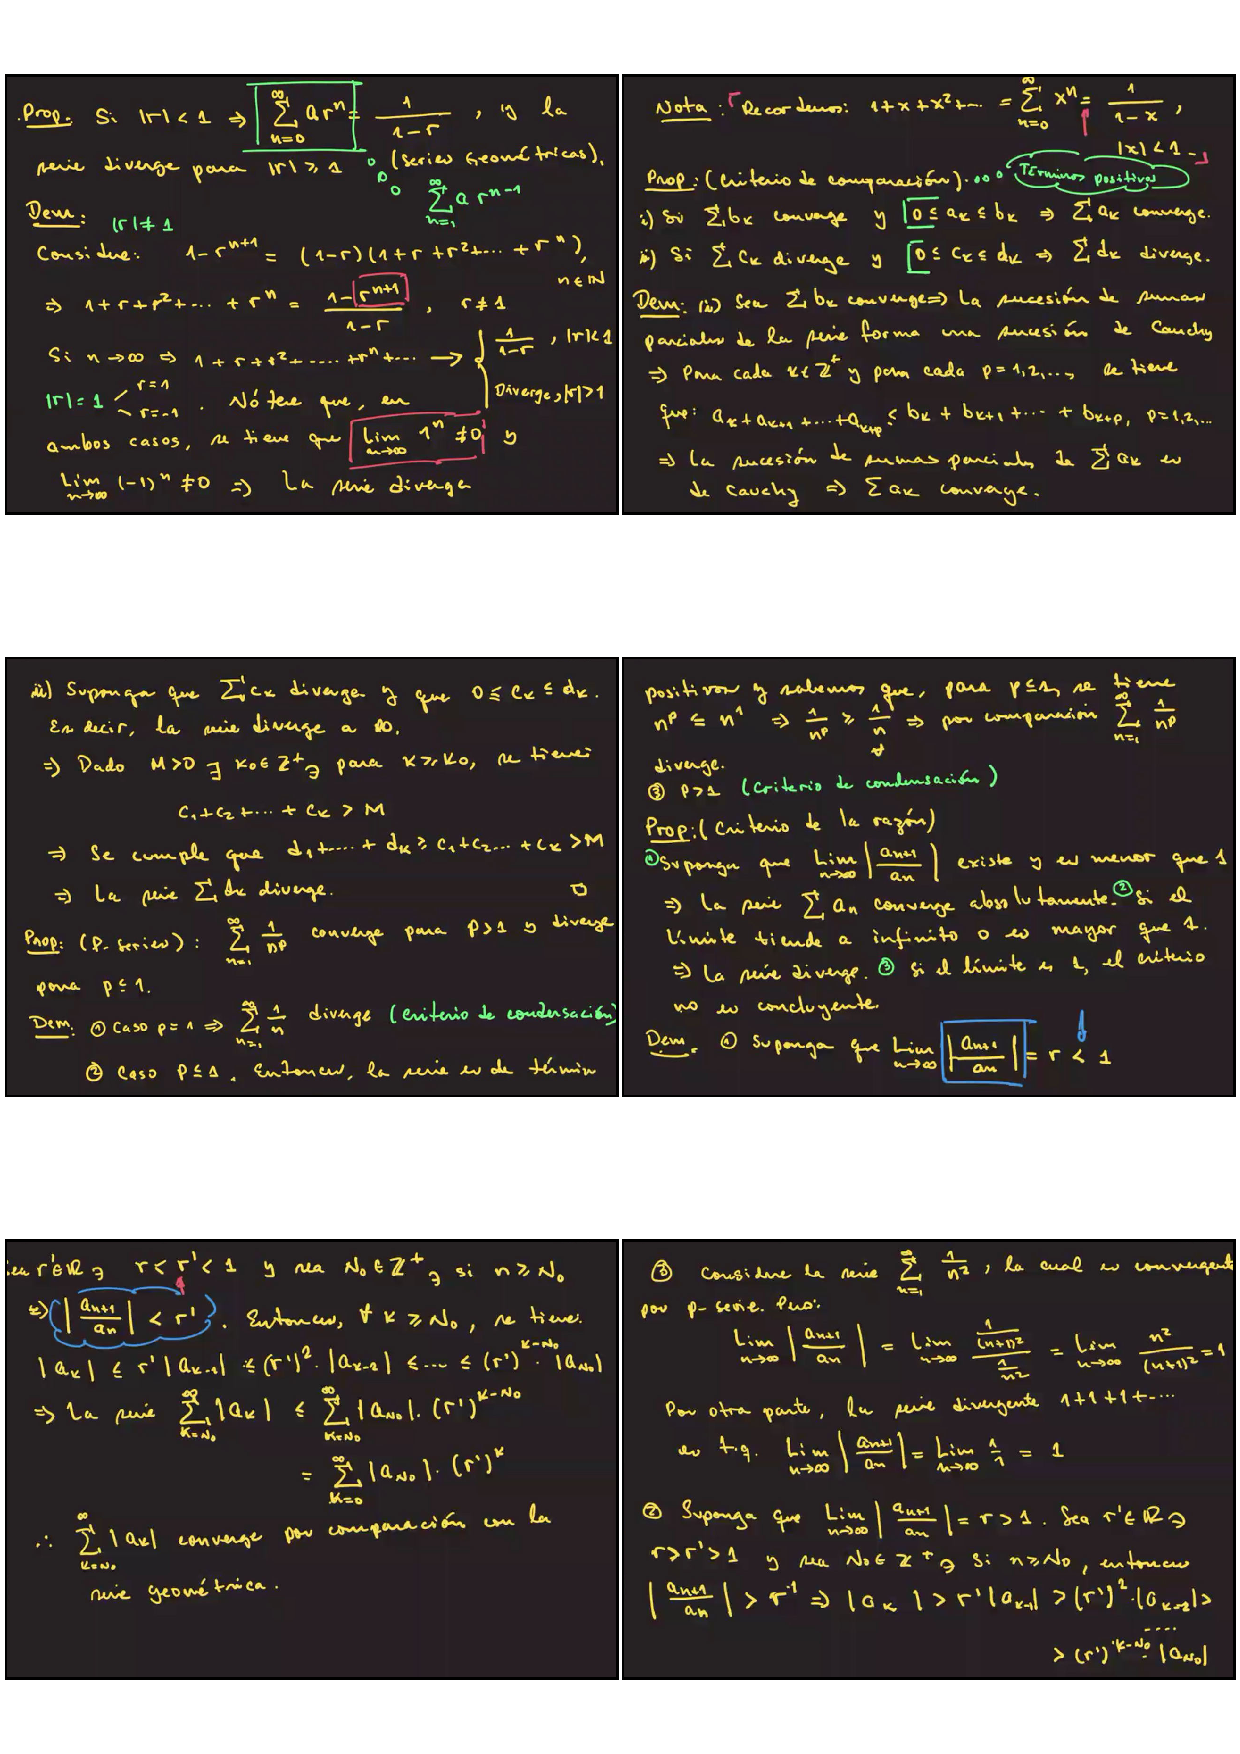
\includepdf[pages=-]{apendices/s11ys12.pdf}